\documentclass[11pt]{article}
\usepackage[utf8]{inputenc}
\usepackage[T1]{fontenc}
\usepackage[spanish]{babel}
\usepackage{amsmath, amssymb, amsthm}
\usepackage{braket}
\usepackage{graphicx}
\usepackage[margin=2.5cm]{geometry}
\usepackage{hyperref}

\allowdisplaybreaks

\newcommand{\ii}{\mathrm{i}}
\newcommand{\ee}{\mathrm{e}}
\newcommand{\dd}{\mathrm{d}}
\newcommand{\vb}[1]{\mathbf{#1}}
\newcommand{\adag}{\hat a^\dagger}
\newcommand{\Ezero}{\mathcal E_0}
\newcommand{\Real}{\operatorname{Re}}
\newcommand{\Imag}{\operatorname{Im}}

\title{Estados del campo electromagn\'etico}
\author{Ricardo Del Rosal Gardu\~no \\ \small Doctorado en F\'isica, BUAP}
\date{Notas a partir de Schleich, \emph{Quantum Optics in Phase Space}}

\begin{document}
\maketitle

\section{Convenci\'on de un solo modo}

Despu\'es de cuantizar el campo electromagn\'etico, cada modo normal del campo
queda descrito por un oscilador arm\'onico cu\'antico. En esta nota se estudia
un solo modo, por lo que se omite el \'indice de modo $\lambda$. Esta
simplificaci\'on permite concentrarse en la estructura cu\'antica del estado
del campo sin cargar la notaci\'on con sumas sobre modos y polarizaciones.

Para un solo modo, el operador de campo el\'ectrico puede escribirse como
\begin{equation}
  \hat{\vb E}(\vb r,t)
  =
  \Ezero \vb u(\vb r)
  \frac{\ii}{\sqrt2}
  \left[
    \hat a(0)\ee^{-\ii\omega t}
    -
    \adag(0)\ee^{\ii\omega t}
  \right].
\end{equation}
Equivalentemente, si se introduce la cuadratura de momento del campo,
\begin{equation}
  \hat\Pi(t)
  =
  \frac{\ii}{\sqrt2}
  \left[
    \adag(0)\ee^{\ii\omega t}
    -
    \hat a(0)\ee^{-\ii\omega t}
  \right],
\end{equation}
entonces
\begin{equation}
  \hat{\vb E}(\vb r,t)
  =
  -\Ezero \vb u(\vb r)\hat\Pi(t).
\end{equation}
La constante $\Ezero$ fija la escala del campo de un fot\'on y
$\vb u(\vb r)$ contiene la forma espacial del modo. La parte no trivial de la
estad\'istica cu\'antica queda, por tanto, en los operadores
$\hat a$ y $\adag$.

\section{Estados de n\'umero de fotones}

Los estados de n\'umero, o estados de Fock, son los eigenestados del operador
n\'umero
\begin{equation}
  \hat n=\adag \hat a,
  \qquad
  \hat n\ket{n}=n\ket{n}.
\end{equation}
Son el an\'alogo cu\'antico de los eigenestados de energ\'ia del oscilador
arm\'onico. Sus reglas de escalera son
\begin{equation}
  \hat a\ket{n}=\sqrt n\,\ket{n-1},
  \qquad
  \adag\ket{n}=\sqrt{n+1}\,\ket{n+1}.
\end{equation}
Estas ecuaciones expresan que $\hat a$ elimina un fot\'on del modo y
$\adag$ crea un fot\'on.

El valor esperado del campo el\'ectrico en el estado $\ket n$ se obtiene
sustituyendo el operador de campo:
\begin{align}
  \langle \hat{\vb E}(\vb r,t)\rangle_n
  &=
  \bra n \hat{\vb E}(\vb r,t)\ket n \notag\\
  &=
  \Ezero\vb u(\vb r)\frac{\ii}{\sqrt2}
  \left[
    \bra n\hat a(0)\ket n\,\ee^{-\ii\omega t}
    -
    \bra n\adag(0)\ket n\,\ee^{\ii\omega t}
  \right].
\end{align}
Usando las reglas de escalera,
\begin{equation}
  \bra n\hat a\ket n
  =
  \sqrt n\,\braket{n|n-1}
  =
  0,
  \qquad
  \bra n\adag\ket n
  =
  \sqrt{n+1}\,\braket{n|n+1}
  =
  0.
\end{equation}
La cancelaci\'on no es din\'amica sino geom\'etrica: $\hat a\ket n$ y
$\adag\ket n$ producen estados ortogonales a $\ket n$. Por tanto,
\begin{equation}
  \boxed{\langle \hat{\vb E}(\vb r,t)\rangle_n=0.}
\end{equation}
Un estado de n\'umero tiene energ\'ia bien definida, pero no tiene una fase de
campo definida. Por eso el campo promedio se anula.

La intensidad del campo no est\'a gobernada por $\hat{\vb E}$ sino por
$\hat{\vb E}^{\,2}$. Para simplificar la notaci\'on se deja impl\'icita la
dependencia temporal de $\hat a(t)=\hat a(0)\ee^{-\ii\omega t}$. Entonces
\begin{align}
  \hat{\vb E}^{\,2}
  &=
  -\frac12 \Ezero^2\vb u^2(\vb r)
  \left(\hat a\ee^{-\ii\omega t}
  -
  \adag\ee^{\ii\omega t}\right)^2 \notag\\
  &=
  -\frac12 \Ezero^2\vb u^2(\vb r)
  \left[
    \hat a^2\ee^{-2\ii\omega t}
    -
    \hat a\adag
    -
    \adag\hat a
    +
    \adag{}^2\ee^{2\ii\omega t}
  \right].
\end{align}
Al tomar el valor esperado en $\ket n$, los t\'erminos $\hat a^2$ y
$\adag{}^2$ no contribuyen porque conectan $\ket n$ con $\ket{n-2}$ y
$\ket{n+2}$:
\begin{equation}
  \bra n \hat a^2\ket n=0,
  \qquad
  \bra n \adag{}^2\ket n=0.
\end{equation}
Los t\'erminos restantes se eval\'uan con
\begin{equation}
  \hat a\adag=\adag\hat a+1=\hat n+1,
  \qquad
  \adag\hat a=\hat n.
\end{equation}
Por tanto,
\begin{align}
  \langle \hat{\vb E}^{\,2}(\vb r,t)\rangle_n
  &=
  \frac12 \Ezero^2\vb u^2(\vb r)
  \bra n
  \left(\hat a\adag+\adag\hat a\right)
  \ket n \notag\\
  &=
  \frac12 \Ezero^2\vb u^2(\vb r)
  \left[(n+1)+n\right].
\end{align}
As\'i se obtiene
\begin{equation}
  \boxed{
  \langle \hat{\vb E}^{\,2}(\vb r,t)\rangle_n
  =
  \Ezero^2\vb u^2(\vb r)\left(n+\frac12\right).
  }
\end{equation}
La intensidad crece linealmente con el n\'umero de fotones. Sin embargo,
queda un t\'ermino incluso cuando $n=0$.

Para el vac\'io,
\begin{equation}
  \langle 0|\hat{\vb E}^{\,2}|0\rangle
  =
  \frac12 \Ezero^2\vb u^2(\vb r).
\end{equation}
Aunque $\langle \hat{\vb E}\rangle_0=0$, el campo no es cl\'asicamente nulo:
presenta fluctuaciones de punto cero. Definiendo un campo efectivo de vac\'io
por unidad de amplitud espacial,
\begin{equation}
  \frac{E_{\mathrm{ef}}}{|\vb u(\vb r)|}
  =
  \left[
  \frac{\langle 0|\hat{\vb E}^{\,2}|0\rangle}{\vb u^2(\vb r)}
  \right]^{1/2},
\end{equation}
se obtiene
\begin{equation}
  \boxed{
  \frac{E_{\mathrm{ef}}}{|\vb u(\vb r)|}
  =
  \frac{\Ezero}{\sqrt2}.
  }
\end{equation}
Estas son las fluctuaciones cu\'anticas del vac\'io. No corresponden a un
campo cl\'asico oscilante, sino al ruido inevitable de la cuadratura del modo.

\section{Eigenestados del campo de radiaci\'on}

Sea $\theta=\omega t$. Se introducen las cuadraturas adimensionales
\begin{equation}
  \hat X=\frac{1}{\sqrt2}(\hat a+\adag),
  \qquad
  \hat\Pi=\frac{\ii}{\sqrt2}(\adag-\hat a),
\end{equation}
que satisfacen $[\hat X,\hat\Pi]=\ii$. La cuadratura rotada del campo se
define como
\begin{equation}
  \hat\varepsilon_\theta
  =
  \hat X\cos\theta+\hat\Pi\sin\theta.
\end{equation}
Al sustituir $\hat X$ y $\hat\Pi$,
\begin{align}
  \hat\varepsilon_\theta
  &=
  \frac{1}{\sqrt2}(\adag+\hat a)\cos\theta
  +
  \frac{\ii}{\sqrt2}(\adag-\hat a)\sin\theta \notag\\
  &=
  \frac{1}{\sqrt2}
  \left[
    \adag(\cos\theta+\ii\sin\theta)
    +
    \hat a(\cos\theta-\ii\sin\theta)
  \right] \notag\\
  &=
  \frac{1}{\sqrt2}
  \left(\adag\ee^{\ii\theta}+\hat a\ee^{-\ii\theta}\right).
\end{align}
Para $\theta=0$ se tiene $\hat\varepsilon_0=\hat X$, mientras que para
$\theta=\pi/2$ se tiene $\hat\varepsilon_{\pi/2}=\hat\Pi$.

Los eigenestados de esta cuadratura se definen por
\begin{equation}
  \hat\varepsilon_\theta\ket{\varepsilon_\theta}
  =
  \varepsilon_\theta\ket{\varepsilon_\theta}.
\end{equation}
Como la base de n\'umero es completa, se expanden como
\begin{equation}
  \ket{\varepsilon_\theta}
  =
  \sum_{n=0}^{\infty}
  \braket{n|\varepsilon_\theta}\ket n.
\end{equation}
Para $\theta=0$ estos coeficientes son las funciones propias del oscilador en
representaci\'on de posici\'on:
\begin{equation}
  \braket{n|\varepsilon_0}
  =
  \pi^{-1/4}
  \frac{1}{\sqrt{2^n n!}}\,
  H_n(\varepsilon_0)\,
  \ee^{-\varepsilon_0^2/2},
\end{equation}
donde $H_n$ son los polinomios de Hermite. Para una cuadratura rotada, aparece
una fase $e^{\ii n\theta}$ en cada componente de n\'umero:
\begin{equation}
  \boxed{
  \ket{\varepsilon_\theta}
  =
  \pi^{-1/4}\ee^{-\varepsilon_\theta^2/2}
  \sum_{n=0}^{\infty}
  \frac{H_n(\varepsilon_\theta)\ee^{\ii n\theta}}
       {\sqrt{2^n n!}}\ket n.
  }
\end{equation}
Esta es la representaci\'on en estados de n\'umero de un eigenestado del campo
de radiaci\'on.

\section{Verificaci\'on de la ecuaci\'on de eigenvalores}

Se verifica ahora que el estado anterior satisface la ecuaci\'on de
eigenvalores. La acci\'on de $\hat\varepsilon_\theta$ sobre $\ket n$ es
\begin{align}
  \hat\varepsilon_\theta\ket n
  &=
  \frac{1}{\sqrt2}
  \left(
    \adag\ee^{\ii\theta}
    +
    \hat a\ee^{-\ii\theta}
  \right)\ket n \notag\\
  &=
  \frac{1}{\sqrt2}
  \left(
    \sqrt{n+1}\,\ee^{\ii\theta}\ket{n+1}
    +
    \sqrt n\,\ee^{-\ii\theta}\ket{n-1}
  \right).
\end{align}
Aplicando esto a la expansi\'on de $\ket{\varepsilon_\theta}$,
\begin{align}
  \hat\varepsilon_\theta\ket{\varepsilon_\theta}
  &=
  \pi^{-1/4}\ee^{-\varepsilon_\theta^2/2}
  \sum_{n=0}^{\infty}
  \frac{H_n(\varepsilon_\theta)\ee^{\ii n\theta}}
       {\sqrt{2^n n!}}\,
  \hat\varepsilon_\theta\ket n \notag\\
  &=
  \pi^{-1/4}\ee^{-\varepsilon_\theta^2/2}
  \left[
  \sum_{n=1}^{\infty}
  \frac{\sqrt n\,H_n(\varepsilon_\theta)\ee^{\ii(n-1)\theta}}
       {\sqrt{2^{n+1}n!}}\ket{n-1}
  \right. \notag\\
  &\hspace{4.5cm}\left.
  +
  \sum_{n=0}^{\infty}
  \frac{\sqrt{n+1}\,H_n(\varepsilon_\theta)\ee^{\ii(n+1)\theta}}
       {\sqrt{2^{n+1}n!}}\ket{n+1}
  \right].
\end{align}
En la primera suma se toma $m=n-1$; en la segunda, $m=n+1$. Entonces ambas
quedan escritas sobre la misma base $\ket m$:
\begin{align}
  \hat\varepsilon_\theta\ket{\varepsilon_\theta}
  &=
  \pi^{-1/4}\ee^{-\varepsilon_\theta^2/2}
  \sum_{m=0}^{\infty}
  \frac{\ee^{\ii m\theta}}{\sqrt{2^m m!}}
  \left[
    \frac12 H_{m+1}(\varepsilon_\theta)
    +
    mH_{m-1}(\varepsilon_\theta)
  \right]\ket m.
\end{align}
La recurrencia de los polinomios de Hermite es
\begin{equation}
  H_{m+1}(z)=2zH_m(z)-2mH_{m-1}(z).
\end{equation}
Por tanto,
\begin{equation}
  \frac12 H_{m+1}(\varepsilon_\theta)
  =
  \varepsilon_\theta H_m(\varepsilon_\theta)
  -
  mH_{m-1}(\varepsilon_\theta).
\end{equation}
Sustituyendo en el corchete, los t\'erminos proporcionales a
$mH_{m-1}$ se cancelan y queda
\begin{equation}
  \hat\varepsilon_\theta\ket{\varepsilon_\theta}
  =
  \varepsilon_\theta
  \pi^{-1/4}\ee^{-\varepsilon_\theta^2/2}
  \sum_{m=0}^{\infty}
  \frac{H_m(\varepsilon_\theta)\ee^{\ii m\theta}}
       {\sqrt{2^m m!}}\ket m.
\end{equation}
As\'i,
\begin{equation}
  \boxed{
  \hat\varepsilon_\theta\ket{\varepsilon_\theta}
  =
  \varepsilon_\theta\ket{\varepsilon_\theta}.
  }
\end{equation}

\section{Por qu\'e un eigenestado de campo no es un campo cl\'asico}

Un eigenestado $\ket{\varepsilon_\theta}$ tiene una cuadratura perfectamente
definida. Por ejemplo, si $\theta=0$, se conoce exactamente $\hat X$; si
$\theta=\pi/2$, se conoce exactamente $\hat\Pi$. Sin embargo, como
\begin{equation}
  [\hat X,\hat\Pi]=\ii,
\end{equation}
las incertidumbres satisfacen
\begin{equation}
  \Delta X\,\Delta\Pi\ge\frac12.
\end{equation}
Por tanto, al fijar una cuadratura se pierde por completo la informaci\'on
sobre la cuadratura conjugada. Como el campo el\'ectrico y el campo magn\'etico
de un modo son proporcionales a cuadraturas conjugadas, se obtiene una relaci\'on
de incertidumbre de la forma
\begin{equation}
  \Delta \hat E\,\Delta \hat H\ge I,
\end{equation}
donde $I$ depende de las constantes de normalizaci\'on del modo y de los
conmutadores. Esta es la raz\'on f\'isica por la que un eigenestado exacto del
campo de radiaci\'on no se comporta como una onda electromagn\'etica cl\'asica:
un campo cl\'asico monocrom\'atico requiere amplitud y fase simult\'aneamente
bien definidas.

\section{Estados coherentes como vac\'io desplazado}

Los estados coherentes proporcionan el compromiso cu\'antico m\'as cercano al
comportamiento cl\'asico. Se definen mediante el operador de desplazamiento
\begin{equation}
  \hat D(\alpha)
  =
  \ee^{\alpha\adag-\alpha^*\hat a},
  \qquad
  \ket{\alpha}=\hat D(\alpha)\ket0.
\end{equation}
Para conectar esta definici\'on con la expansi\'on en estados de n\'umero se
usa la f\'ormula de Baker-Campbell-Hausdorff,
\begin{equation}
  \ee^{\hat A+\hat B}
  =
  \ee^{\hat A}\ee^{\hat B}\ee^{-[\hat A,\hat B]/2},
\end{equation}
cuando $[\hat A,\hat B]$ conmuta con $\hat A$ y $\hat B$. Tomando
\begin{equation}
  \hat A=\alpha\adag,
  \qquad
  \hat B=-\alpha^*\hat a,
\end{equation}
se tiene
\begin{equation}
  [\hat A,\hat B]
  =
  \alpha(-\alpha^*)[\adag,\hat a]
  =
  |\alpha|^2.
\end{equation}
Como este conmutador es un n\'umero, los conmutadores anidados se anulan.
Entonces
\begin{equation}
  \hat D(\alpha)
  =
  \ee^{-|\alpha|^2/2}
  \ee^{\alpha\adag}
  \ee^{-\alpha^*\hat a}.
\end{equation}
Actuando sobre el vac\'io,
\begin{equation}
  \ee^{-\alpha^*\hat a}\ket0
  =
  \left(
  1-\alpha^*\hat a+\frac{\alpha^{*2}}{2!}\hat a^2-\cdots
  \right)\ket0
  =
  \ket0,
\end{equation}
porque $\hat a\ket0=0$. Por lo tanto,
\begin{align}
  \ket{\alpha}
  &=
  \ee^{-|\alpha|^2/2}
  \ee^{\alpha\adag}\ket0 \notag\\
  &=
  \ee^{-|\alpha|^2/2}
  \sum_{n=0}^{\infty}
  \frac{\alpha^n}{n!}\adag{}^n\ket0.
\end{align}
Como $\adag{}^n\ket0=\sqrt{n!}\ket n$, resulta
\begin{equation}
  \boxed{
  \ket{\alpha}
  =
  \ee^{-|\alpha|^2/2}
  \sum_{n=0}^{\infty}
  \frac{\alpha^n}{\sqrt{n!}}\ket n.
  }
\end{equation}

\section{Estad\'istica de fotones del estado coherente}

La probabilidad de encontrar $n$ fotones en un estado coherente es
\begin{equation}
  W_n
  =
  |\braket{n|\alpha}|^2
  =
  \ee^{-|\alpha|^2}
  \frac{|\alpha|^{2n}}{n!}.
\end{equation}
Esta es una distribuci\'on de Poisson con par\'ametro $|\alpha|^2$.

El n\'umero promedio de fotones es
\begin{align}
  \langle \hat n\rangle
  &=
  \sum_{n=0}^{\infty} nW_n \notag\\
  &=
  \sum_{n=1}^{\infty}
  n\,
  \frac{|\alpha|^{2n}}{n!}\ee^{-|\alpha|^2} \notag\\
  &=
  |\alpha|^2
  \sum_{n=1}^{\infty}
  \frac{|\alpha|^{2(n-1)}}{(n-1)!}\ee^{-|\alpha|^2}.
\end{align}
Con $m=n-1$,
\begin{equation}
  \langle \hat n\rangle
  =
  |\alpha|^2
  \sum_{m=0}^{\infty}
  \frac{|\alpha|^{2m}}{m!}\ee^{-|\alpha|^2}
  =
  |\alpha|^2,
\end{equation}
pues la suma es $\ee^{|\alpha|^2}\ee^{-|\alpha|^2}=1$.
El par\'ametro $|\alpha|^2$ es, entonces, el n\'umero promedio de fotones.

Para hallar el ancho de la distribuci\'on se calcula la varianza
\begin{equation}
  \sigma^2
  =
  \langle \hat n^2\rangle-\langle\hat n\rangle^2.
\end{equation}
Primero,
\begin{align}
  \langle\hat n^2\rangle
  &=
  \sum_{n=0}^{\infty}
  n^2
  \frac{|\alpha|^{2n}}{n!}\ee^{-|\alpha|^2} \notag\\
  &=
  \sum_{n=1}^{\infty}
  n
  \frac{|\alpha|^{2n}}{(n-1)!}\ee^{-|\alpha|^2}.
\end{align}
Escribiendo $n=(n-1)+1$,
\begin{align}
  \langle\hat n^2\rangle
  &=
  \sum_{n=1}^{\infty}
  (n-1)
  \frac{|\alpha|^{2n}}{(n-1)!}\ee^{-|\alpha|^2}
  +
  \sum_{n=1}^{\infty}
  \frac{|\alpha|^{2n}}{(n-1)!}\ee^{-|\alpha|^2} \notag\\
  &=
  |\alpha|^4
  \sum_{m=0}^{\infty}
  \frac{|\alpha|^{2m}}{m!}\ee^{-|\alpha|^2}
  +
  |\alpha|^2
  \sum_{m=0}^{\infty}
  \frac{|\alpha|^{2m}}{m!}\ee^{-|\alpha|^2}.
\end{align}
Por tanto,
\begin{equation}
  \langle\hat n^2\rangle=|\alpha|^4+|\alpha|^2,
  \qquad
  \boxed{\sigma^2=|\alpha|^2.}
\end{equation}
La desviaci\'on est\'andar es
\begin{equation}
  \sigma=\sqrt{|\alpha|^2}=\sqrt{\langle\hat n\rangle}.
\end{equation}
Al aumentar el n\'umero medio de fotones, el ancho absoluto crece, pero el
ancho relativo decrece:
\begin{equation}
  \frac{\sigma}{\langle\hat n\rangle}
  =
  \frac{1}{\sqrt{\langle\hat n\rangle}}
  \xrightarrow{\langle\hat n\rangle\to\infty}0.
\end{equation}
Este es uno de los sentidos precisos en los que el estado coherente se acerca
al comportamiento cl\'asico para intensidades grandes.

El mismo resultado puede verse directamente usando
$\hat a\ket\alpha=\alpha\ket\alpha$:
\begin{equation}
  \langle\hat n\rangle
  =
  \bra\alpha\adag\hat a\ket\alpha
  =
  \alpha^*\alpha
  =
  |\alpha|^2.
\end{equation}
Adem\'as,
\begin{align}
  \langle\hat n^2\rangle
  &=
  \bra\alpha\adag\hat a\adag\hat a\ket\alpha \notag\\
  &=
  \bra\alpha\adag(\adag\hat a+1)\hat a\ket\alpha \notag\\
  &=
  \bra\alpha\adag{}^2\hat a^2\ket\alpha
  +
  \bra\alpha\adag\hat a\ket\alpha \notag\\
  &=
  |\alpha|^4+|\alpha|^2.
\end{align}
La parte adicional $|\alpha|^2$ aparece por el conmutador
$[\hat a,\adag]=1$.

\section{Distribuci\'on del campo el\'ectrico en un estado coherente}

La probabilidad de encontrar el valor $\varepsilon_\theta$ de la cuadratura
del campo cuando el modo est\'a en el estado coherente $\ket\beta$ es
\begin{equation}
  W_{\ket\beta}(\varepsilon_\theta)
  =
  |\braket{\varepsilon_\theta|\beta}|^2.
\end{equation}
Usando la representaci\'on de n\'umero,
\begin{equation}
  \bra{\varepsilon_\theta}
  =
  \pi^{-1/4}\ee^{-\varepsilon_\theta^2/2}
  \sum_{n=0}^{\infty}
  \frac{H_n(\varepsilon_\theta)\ee^{-\ii n\theta}}
       {\sqrt{2^n n!}}\bra n,
\end{equation}
y
\begin{equation}
  \ket\beta
  =
  \ee^{-|\beta|^2/2}
  \sum_{n=0}^{\infty}\frac{\beta^n}{\sqrt{n!}}\ket n,
\end{equation}
se obtiene
\begin{align}
  \braket{\varepsilon_\theta|\beta}
  &=
  \pi^{-1/4}
  \ee^{-\varepsilon_\theta^2/2}
  \ee^{-|\beta|^2/2}
  \sum_{n=0}^{\infty}
  \frac{H_n(\varepsilon_\theta)}{n!}
  \left(\frac{\beta\ee^{-\ii\theta}}{\sqrt2}\right)^n.
\end{align}
La funci\'on generatriz de los polinomios de Hermite,
\begin{equation}
  \sum_{n=0}^{\infty}\frac{z^n}{n!}H_n(\xi)
  =
  \ee^{-z^2+2\xi z},
\end{equation}
con
\begin{equation}
  z=\frac{\beta\ee^{-\ii\theta}}{\sqrt2},
\end{equation}
da
\begin{equation}
  \braket{\varepsilon_\theta|\beta}
  =
  \pi^{-1/4}
  \exp\left[
  -\frac12\varepsilon_\theta^2
  -\frac12(\beta\ee^{-\ii\theta})^2
  +\sqrt2\,\varepsilon_\theta\beta\ee^{-\ii\theta}
  -\frac12|\beta|^2
  \right].
\end{equation}
Para $\theta=0$ y $\beta$ real, esta expresi\'on se reduce a
\begin{equation}
  \braket{x|\beta}
  =
  \pi^{-1/4}
  \exp\left[
  \frac12(\beta^2-|\beta|^2)
  \right]
  \exp\left[-\frac12(x-\sqrt2\,\beta)^2\right].
\end{equation}
Si $\beta$ es real, el prefactor de fase se cancela. Si $\beta$ es complejo,
ese factor de fase es importante, especialmente cuando se superponen estados
coherentes.

Tomando el m\'odulo cuadrado de la amplitud general,
\begin{equation}
  \boxed{
  W_{\ket\beta}(\varepsilon_\theta)
  =
  \pi^{-1/2}
  \exp\left[
  -\left(
  \varepsilon_\theta
  -
  \frac{1}{\sqrt2}
  \left(
  \beta\ee^{-\ii\theta}
  +
  \beta^*\ee^{\ii\theta}
  \right)
  \right)^2
  \right].
  }
\end{equation}
Es una gaussiana centrada en
\begin{equation}
  \varepsilon_\theta^{(0)}
  =
  \frac{1}{\sqrt2}
  \left(
  \beta\ee^{-\ii\theta}
  +
  \beta^*\ee^{\ii\theta}
  \right)
  =
  \sqrt2\,\Real(\beta\ee^{-\ii\theta}).
\end{equation}
El estado coherente desplaza el centro de la distribuci\'on del vac\'io sin
cambiar su anchura.

\section{Sobre-completitud de los estados coherentes}

Los estados coherentes forman un conjunto sobre-completo: su conjunto es
completo, pero no ortogonal. La relaci\'on de identidad es
\begin{equation}
  \boxed{
  \hat I
  =
  \frac1\pi\int \dd^2\alpha\,\ket\alpha\bra\alpha.
  }
\end{equation}
Aqu\'i $\alpha=|\alpha|\ee^{\ii\theta}$ y el elemento de \'area en el plano
complejo es
\begin{equation}
  \dd^2\alpha
  =
  \dd(\Real\alpha)\dd(\Imag\alpha)
  =
  |\alpha|\,\dd|\alpha|\,\dd\theta.
\end{equation}

Para demostrar la identidad se sustituye la expansi\'on en estados de n\'umero:
\begin{align}
  \frac1\pi\int\dd^2\alpha\,\ket\alpha\bra\alpha
  &=
  \frac1\pi
  \int_0^\infty |\alpha|\dd|\alpha|
  \int_0^{2\pi}\dd\theta\,
  \ee^{-|\alpha|^2}
  \sum_{n,m=0}^{\infty}
  \frac{\alpha^n(\alpha^*)^m}{\sqrt{n!m!}}
  \ket n\bra m.
\end{align}
Como $\alpha^n(\alpha^*)^m=|\alpha|^{n+m}\ee^{\ii(n-m)\theta}$,
\begin{align}
  \frac1\pi\int\dd^2\alpha\,\ket\alpha\bra\alpha
  &=
  \sum_{n,m=0}^{\infty}
  \frac{\ket n\bra m}{\sqrt{n!m!}}
  \int_0^\infty |\alpha|^{n+m+1}\ee^{-|\alpha|^2}\dd|\alpha|
  \frac1\pi\int_0^{2\pi}\ee^{\ii(n-m)\theta}\dd\theta.
\end{align}
La integral angular es
\begin{equation}
  \int_0^{2\pi}\ee^{\ii(n-m)\theta}\dd\theta
  =
  2\pi\,\delta_{nm}.
\end{equation}
Por eso s\'olo sobreviven los t\'erminos diagonales $n=m$:
\begin{align}
  \frac1\pi\int\dd^2\alpha\,\ket\alpha\bra\alpha
  &=
  \sum_{n=0}^{\infty}
  \frac{2}{n!}
  \int_0^\infty
  |\alpha|^{2n+1}\ee^{-|\alpha|^2}\dd|\alpha|
  \ket n\bra n.
\end{align}
Con $u=|\alpha|^2$, $\dd u=2|\alpha|\dd|\alpha|$, se obtiene
\begin{equation}
  2\int_0^\infty
  |\alpha|^{2n+1}\ee^{-|\alpha|^2}\dd|\alpha|
  =
  \int_0^\infty u^n\ee^{-u}\dd u
  =
  \Gamma(n+1)=n!.
\end{equation}
As\'i,
\begin{equation}
  \frac1\pi\int\dd^2\alpha\,\ket\alpha\bra\alpha
  =
  \sum_{n=0}^{\infty}\ket n\bra n
  =
  \hat I.
\end{equation}

La no ortogonalidad se obtiene calculando el traslape de dos estados
coherentes:
\begin{align}
  \braket{\alpha|\beta}
  &=
  \ee^{-\frac12(|\alpha|^2+|\beta|^2)}
  \sum_{n=0}^{\infty}
  \frac{(\alpha^*\beta)^n}{n!} \notag\\
  &=
  \boxed{
  \exp\left[
  -\frac12(|\alpha|^2+|\beta|^2)+\alpha^*\beta
  \right].
  }
\end{align}
Su m\'odulo cuadrado es
\begin{equation}
  \boxed{
  |\braket{\alpha|\beta}|^2
  =
  \ee^{-|\alpha-\beta|^2}.
  }
\end{equation}
El traslape entre dos estados coherentes es una gaussiana en la separaci\'on
entre sus puntos del espacio fase. Mientras mayor sea la separaci\'on, menor
ser\'a el traslape.

\section{Expansi\'on en estados coherentes}

Una consecuencia directa de la sobre-completitud es que cualquier estado puede
expandirse en estados coherentes. En particular,
\begin{align}
  \ket\alpha
  &=
  \hat I\ket\alpha \notag\\
  &=
  \frac1\pi\int\dd^2\beta\,\ket\beta\braket{\beta|\alpha} \notag\\
  &=
  \frac1\pi\int\dd^2\beta\,
  \exp\left[
  -\frac12(|\alpha|^2+|\beta|^2)+\beta^*\alpha
  \right]\ket\beta.
\end{align}
El factor de peso se puede escribir como
\begin{equation}
  \exp\left[
  -\frac12|\alpha-\beta|^2
  \right]
  \exp[\ii\Phi(\beta;\alpha)],
  \qquad
  \Phi(\beta;\alpha)=\Imag(\alpha\beta^*).
\end{equation}
La parte gaussiana mide la separaci\'on entre el estado coherente que se
expande y el estado coherente $\ket\beta$ usado en la superposici\'on. La fase
$\Phi$ contiene el \'area orientada asociada al tri\'angulo formado por el
origen y los puntos complejos $\alpha$ y $\beta$.

Tambi\'en puede expandirse un estado de n\'umero en estados coherentes. En
vez de integrar sobre todo el plano complejo, basta integrar sobre un c\'irculo
de radio fijo $|\beta|$. Se parte de
\begin{equation}
  \ket{|\beta|\ee^{\ii\theta}}
  =
  \ee^{-|\beta|^2/2}
  \sum_{m=0}^{\infty}
  \frac{|\beta|^m\ee^{\ii m\theta}}{\sqrt{m!}}\ket m.
\end{equation}
Multiplicando por $\ee^{-\ii n\theta}$ e integrando,
\begin{align}
  \frac1{2\pi}\int_0^{2\pi}
  \ee^{-\ii n\theta}\ket{|\beta|\ee^{\ii\theta}}\dd\theta
  &=
  \ee^{-|\beta|^2/2}
  \sum_{m=0}^{\infty}
  \frac{|\beta|^m}{\sqrt{m!}}
  \left[
  \frac1{2\pi}
  \int_0^{2\pi}\ee^{\ii(m-n)\theta}\dd\theta
  \right]\ket m \notag\\
  &=
  \ee^{-|\beta|^2/2}
  \frac{|\beta|^n}{\sqrt{n!}}\ket n.
\end{align}
Por tanto,
\begin{equation}
  \boxed{
  \ket n
  =
  \ee^{|\beta|^2/2}
  \frac{\sqrt{n!}}{|\beta|^n}
  \frac1{2\pi}
  \int_0^{2\pi}
  \ee^{-\ii n\theta}\ket{|\beta|\ee^{\ii\theta}}\dd\theta.
  }
\end{equation}
Esta expresi\'on muestra que un estado de n\'umero se obtiene como una
superposici\'on continua de estados coherentes distribuidos sobre un c\'irculo
de radio fijo en el espacio fase.

\section{Valores esperados del campo el\'ectrico en estados coherentes}

Para un solo modo,
\begin{equation}
  \hat{\vb E}
  =
  \Ezero\vb u(\vb r)\frac{\ii}{\sqrt2}
  \left[\hat a(t)-\adag(t)\right].
\end{equation}
Si el estado es coherente,
\begin{equation}
  \hat a(t)\ket\alpha=\alpha(t)\ket\alpha,
  \qquad
  \alpha(t)=\alpha(0)\ee^{-\ii\omega t}.
\end{equation}
Entonces
\begin{align}
  \langle\hat{\vb E}\rangle_\alpha
  &=
  \Ezero\vb u(\vb r)\frac{\ii}{\sqrt2}
  \left[
  \alpha(t)-\alpha^*(t)
  \right] \notag\\
  &=
  -\sqrt2\,\Ezero\vb u(\vb r)\,\Imag[\alpha(t)].
\end{align}
Si $\alpha(t)=|\alpha|\ee^{\ii\Theta(t)}$,
\begin{equation}
  \boxed{
  \langle\hat{\vb E}\rangle_\alpha
  =
  -\sqrt2\,\Ezero\vb u(\vb r)|\alpha|\sin\Theta(t).
  }
\end{equation}
Esta es precisamente la forma de un campo el\'ectrico cl\'asico
monocrom\'atico con amplitud proporcional a $\sqrt2\,\Ezero|\alpha|$ y fase
$\Theta(t)$.

Ahora se calcula $\langle\hat{\vb E}^{\,2}\rangle_\alpha$:
\begin{align}
  \langle\hat{\vb E}^{\,2}\rangle_\alpha
  &=
  -\frac12\Ezero^2\vb u^2(\vb r)
  \bra\alpha(\hat a-\adag)^2\ket\alpha \notag\\
  &=
  -\frac12\Ezero^2\vb u^2(\vb r)
  \bra\alpha
  \left(
  \hat a^2+\adag{}^2-2\adag\hat a-1
  \right)
  \ket\alpha \notag\\
  &=
  -\frac12\Ezero^2\vb u^2(\vb r)
  \left[
  \alpha^2+\alpha^{*2}-2|\alpha|^2-1
  \right] \notag\\
  &=
  -\frac12\Ezero^2\vb u^2(\vb r)
  \left[
  (\alpha-\alpha^*)^2-1
  \right].
\end{align}
Como
\begin{equation}
  \langle\hat{\vb E}\rangle_\alpha^2
  =
  -\frac12\Ezero^2\vb u^2(\vb r)(\alpha-\alpha^*)^2,
\end{equation}
la varianza queda
\begin{align}
  \sigma_E^2
  &=
  \langle\hat{\vb E}^{\,2}\rangle_\alpha
  -
  \langle\hat{\vb E}\rangle_\alpha^2 \notag\\
  &=
  \boxed{
  \frac12\Ezero^2\vb u^2(\vb r).
  }
\end{align}
Las fluctuaciones del campo el\'ectrico en un estado coherente son
independientes de $\alpha$. En contraste, para un estado de n\'umero se obtuvo
\begin{equation}
  \sigma_{E,n}^2
  =
  \Ezero^2\vb u^2(\vb r)\left(n+\frac12\right).
\end{equation}
Para $n=0$, las fluctuaciones del vac\'io coinciden con las de un estado
coherente. Por eso los estados coherentes son los m\'as cercanos al caso
cl\'asico: poseen campo medio no nulo y fluctuaciones m\'inimas, iguales a las
del vac\'io.

\section{Estados gato de Schr\"odinger}

Un estado gato de Schr\"odinger de un solo modo se define como una
superposici\'on de dos estados coherentes macrosc\'opicamente distinguibles:
\begin{equation}
  \ket\psi
  =
  N\,\frac{1}{\sqrt2}
  \left(
  \ket{\alpha\ee^{\ii\varphi}}
  +
  \ket{\alpha\ee^{-\ii\varphi}}
  \right),
\end{equation}
donde se toma $\alpha$ real y positiva. Los dos estados coherentes tienen el
mismo m\'odulo, pero fases opuestas. En el plano de cuadraturas sus centros
est\'an en
\begin{equation}
  \langle x\rangle=\sqrt2\,\alpha\cos\varphi,
  \qquad
  \langle p\rangle=\pm\sqrt2\,\alpha\sin\varphi.
\end{equation}
La constante $N$ no es igual a uno porque los estados coherentes no son
ortogonales. Usando
\begin{equation}
  \braket{\alpha|\beta}
  =
  \exp\left[
  -\frac12(|\alpha|^2+|\beta|^2)+\alpha^*\beta
  \right],
\end{equation}
se encuentra
\begin{align}
  1
  &=
  \braket{\psi|\psi} \notag\\
  &=
  \frac{N^2}{2}
  \left[
  2+
  \braket{\alpha\ee^{\ii\varphi}|\alpha\ee^{-\ii\varphi}}
  +
  \braket{\alpha\ee^{-\ii\varphi}|\alpha\ee^{\ii\varphi}}
  \right] \notag\\
  &=
  N^2
  \left[
  1+
  \Real\left(
  \ee^{-\alpha^2+\alpha^2\ee^{-2\ii\varphi}}
  \right)
  \right].
\end{align}
Ahora,
\begin{align}
  \Real\left(
  \ee^{-\alpha^2+\alpha^2\ee^{-2\ii\varphi}}
  \right)
  &=
  \Real\left[
  \ee^{-\alpha^2(1-\cos2\varphi)}
  \ee^{-\ii\alpha^2\sin2\varphi}
  \right] \notag\\
  &=
  \ee^{-2\alpha^2\sin^2\varphi}
  \cos(\alpha^2\sin2\varphi).
\end{align}
Definiendo
\begin{equation}
  P_\varphi=|\sqrt2\,\alpha\sin\varphi|,
\end{equation}
la normalizaci\'on queda
\begin{equation}
  \boxed{
  N^2(\varphi)
  =
  \frac{1}
  {1+\ee^{-P_\varphi^2}\cos(\alpha^2\sin2\varphi)}.
  }
\end{equation}

\section{Funci\'on de Wigner del estado gato}

La funci\'on de Wigner de un estado puro con funci\'on de onda $\psi(x)$ es
\begin{equation}
  W_\psi(x,p)
  =
  \frac1\pi
  \int_{-\infty}^{\infty}
  \dd y\,
  \ee^{2\ii py}\,
  \psi^*(x+y)\psi(x-y).
\end{equation}
Para el estado gato,
\begin{equation}
  \psi(x)=
  \frac{N}{\sqrt2}
  \left[\psi_+(x)+\psi_-(x)\right],
\end{equation}
donde
\begin{equation}
  \psi_\pm(x)
  =
  \braket{x|\alpha\ee^{\pm\ii\varphi}}.
\end{equation}
Por la bilinealidad de la definici\'on de Wigner aparecen cuatro t\'erminos:
\begin{equation}
  W_\psi
  =
  \frac{N^2}{2}
  \left(
  W_{++}+W_{+-}+W_{-+}+W_{--}
  \right).
\end{equation}
Los t\'erminos $W_{++}$ y $W_{--}$ son las contribuciones diagonales de cada
estado coherente por separado. Los t\'erminos cruzados $W_{+-}$ y $W_{-+}$ son
los que producen las franjas de interferencia.

La representaci\'on en posici\'on de un estado coherente centrado en
$(x_0,p_0)$ es
\begin{equation}
  \braket{x|\alpha}
  =
  \pi^{-1/4}
  \exp\left[
  -\frac12(x-x_0)^2
  +\ii xp_0
  -\frac{\ii}{2}x_0p_0
  \right],
\end{equation}
con
\begin{equation}
  x_0=\sqrt2\,\alpha\cos\varphi,
  \qquad
  p_0=\sqrt2\,\alpha\sin\varphi.
\end{equation}
Al calcular, por ejemplo, el t\'ermino cruzado $W_{+-}$, se obtiene una
integral gaussiana:
\begin{align}
  W_{+-}
  &=
  \int_{-\infty}^{\infty}\dd y\,
  \ee^{2\ii py}\psi_+(x+y)\psi_-^*(x-y) \notag\\
  &=
  \pi^{-1/2}
  \int_{-\infty}^{\infty}\dd y\,
  \exp\left[
  2\ii py
  -(x-x_0)^2-y^2
  +2\ii p_0x
  -\ii\alpha^2\sin2\varphi
  \right] \notag\\
  &=
  \ee^{-(x-x_0)^2-p^2}
  \exp\left[
  \ii\left(-\alpha^2\sin2\varphi+2p_0x\right)
  \right].
\end{align}
El otro t\'ermino cruzado es su complejo conjugado,
\begin{equation}
  W_{-+}=W_{+-}^*.
\end{equation}
Al sumarlos aparece un coseno. Los t\'erminos diagonales son
\begin{equation}
  W_{++}
  =
  \ee^{-(x-x_0)^2-(p+p_0)^2},
  \qquad
  W_{--}
  =
  \ee^{-(x-x_0)^2-(p-p_0)^2}.
\end{equation}
Por tanto, la funci\'on completa es
\begin{equation}
  \boxed{
  \begin{aligned}
  W_\psi(x,p)
  &=
  \frac{N^2}{2\pi}
  \left[
  \ee^{-(x-x_0)^2-(p+p_0)^2}
  +
  \ee^{-(x-x_0)^2-(p-p_0)^2}
  \right.\\
  &\hspace{2.4cm}\left.
  +
  2\ee^{-(x-x_0)^2-p^2}
  \cos\left(2p_0x-\alpha^2\sin2\varphi\right)
  \right].
  \end{aligned}
  }
\end{equation}
Con $x_0=\sqrt2\,\alpha\cos\varphi$ y
$p_0=\sqrt2\,\alpha\sin\varphi$, el argumento del coseno tambi\'en puede
escribirse como
\begin{equation}
  2p_0x-\alpha^2\sin2\varphi
  =
  2\sqrt2\,\alpha\sin\varphi
  \left(
  x-\frac{\alpha}{\sqrt2}\cos\varphi
  \right).
\end{equation}
As\'i,
\begin{equation}
  W_\psi(x,p)
  =
  \frac{N^2}{2}
  \left(
  W_{\ket{\alpha\ee^{\ii\varphi}}}
  +
  W_{\ket{\alpha\ee^{-\ii\varphi}}}
  +
  W_{\mathrm{int}}
  \right),
\end{equation}
donde
\begin{equation}
  W_{\ket{\alpha\ee^{\pm\ii\varphi}}}
  =
  \frac1\pi
  \ee^{-(x-\sqrt2\alpha\cos\varphi)^2
  -(p\pm\sqrt2\alpha\sin\varphi)^2},
\end{equation}
y
\begin{equation}
  W_{\mathrm{int}}
  =
  \frac{2}{\pi}
  \ee^{-(x-\sqrt2\alpha\cos\varphi)^2-p^2}
  \cos\left[
  2\sqrt2\,\alpha\sin\varphi
  \left(
  x-\frac{\alpha}{\sqrt2}\cos\varphi
  \right)
  \right].
\end{equation}
Si no existieran los t\'erminos cruzados, la funci\'on de Wigner ser\'ia una
mezcla estad\'istica de dos gaussianas. La presencia de $W_{\mathrm{int}}$
revela que el estado es una superposici\'on coherente: aparecen franjas de
interferencia y la funci\'on de Wigner puede tomar valores negativos.

\begin{figure}[h]
  \centering
  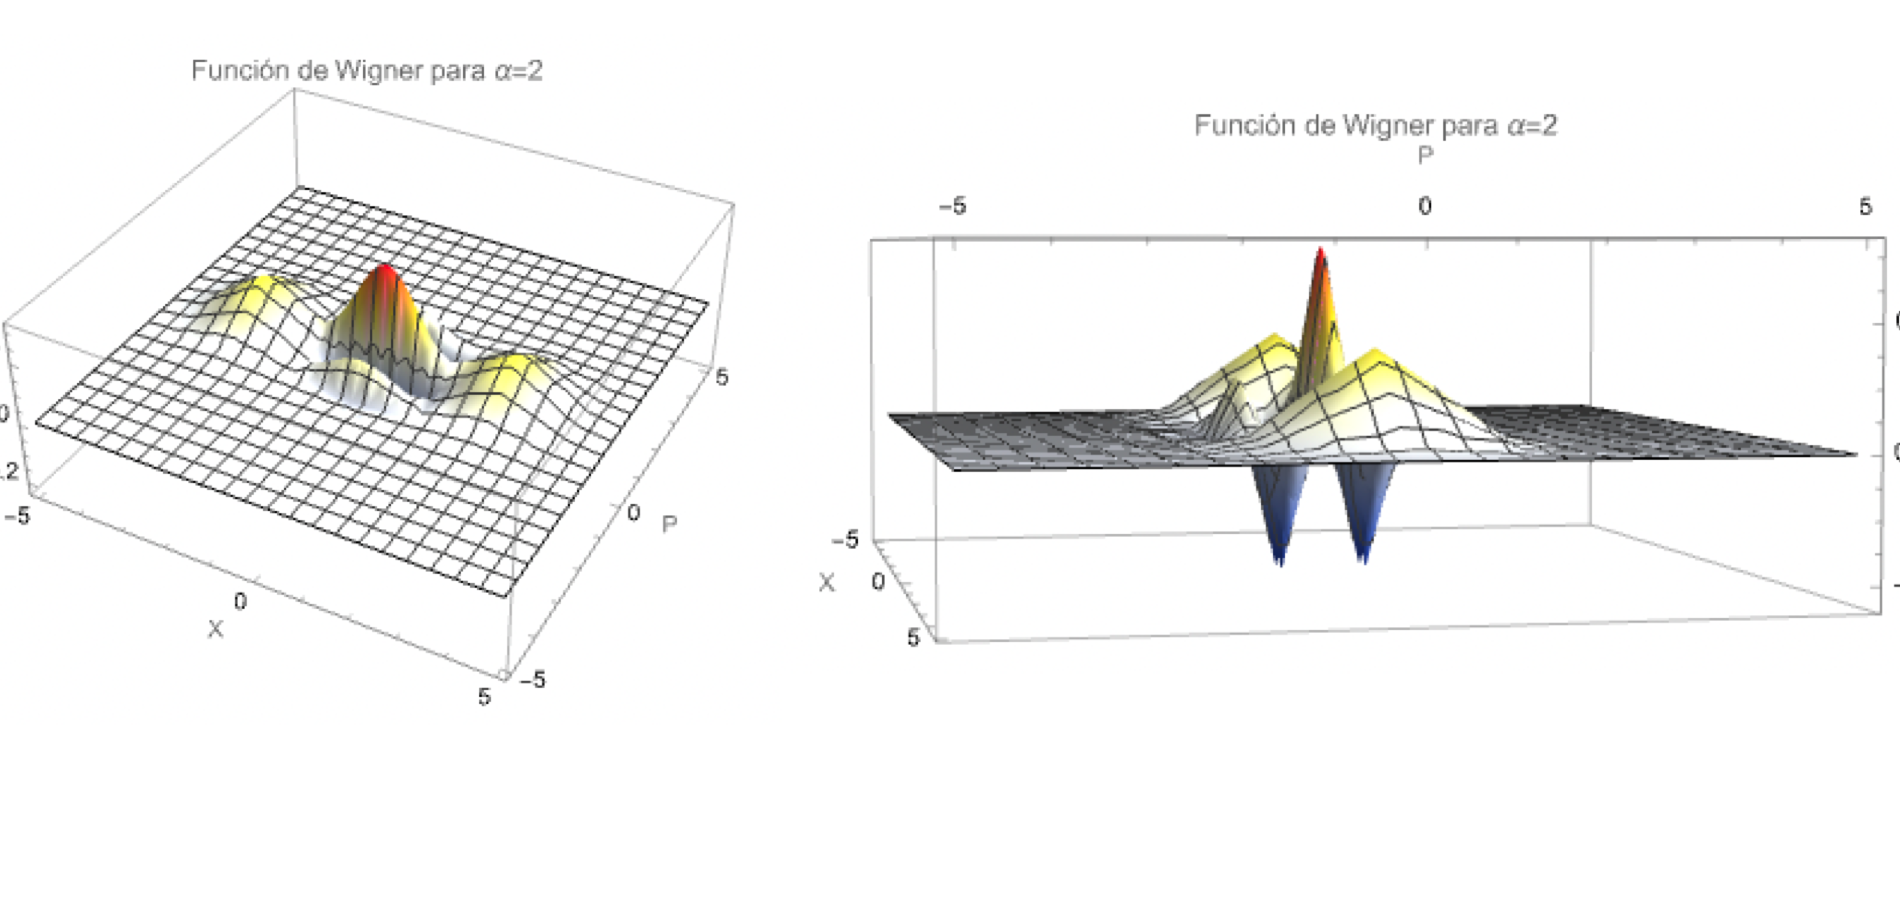
\includegraphics[width=0.92\linewidth]{../../notas-doctorado/imgs/wigner_gato_alpha2.png}
  \caption{Funci\'on de Wigner de una superposici\'on de estados coherentes. Los dos picos corresponden a las componentes coherentes y las franjas centrales corresponden al t\'ermino de interferencia.}
\end{figure}

\section{Estad\'istica de fotones del estado gato}

Finalmente se estudia la probabilidad $W_m$ de hallar $m$ fotones en el estado
gato. A diferencia de la distribuci\'on de Poisson de un solo estado
coherente, ahora la superposici\'on introduce interferencia dependiente de la
diferencia de fase $2\varphi$.

La probabilidad es
\begin{align}
  W_m(\psi)
  &=
  |\braket{m|\psi}|^2 \notag\\
  &=
  \frac{N^2}{2}
  \left|
  \braket{m|\alpha\ee^{\ii\varphi}}
  +
  \braket{m|\alpha\ee^{-\ii\varphi}}
  \right|^2.
\end{align}
Como
\begin{equation}
  \braket{m|\beta}
  =
  \frac{\beta^m}{\sqrt{m!}}\ee^{-|\beta|^2/2},
\end{equation}
entonces
\begin{align}
  W_m(\psi)
  &=
  \frac{N^2}{2}
  \left|
  \frac{\alpha^m}{\sqrt{m!}}\ee^{-\alpha^2/2}\ee^{\ii m\varphi}
  +
  \frac{\alpha^m}{\sqrt{m!}}\ee^{-\alpha^2/2}\ee^{-\ii m\varphi}
  \right|^2 \notag\\
  &=
  \frac{N^2}{2}
  \frac{\alpha^{2m}}{m!}\ee^{-\alpha^2}
  \left|\ee^{\ii m\varphi}+\ee^{-\ii m\varphi}\right|^2 \notag\\
  &=
  2N^2
  \frac{\alpha^{2m}}{m!}\ee^{-\alpha^2}
  \cos^2(m\varphi).
\end{align}
Por tanto,
\begin{equation}
  \boxed{
  W_m(\psi)
  =
  2N^2
  \frac{\alpha^{2m}}{m!}\ee^{-\alpha^2}
  \cos^2(m\varphi).
  }
\end{equation}
Hasta el factor de normalizaci\'on, se obtiene la distribuci\'on de Poisson de
un estado coherente modulada por el factor de interferencia
$\cos^2(m\varphi)$. Esta modulaci\'on puede estrechar o ensanchar la
distribuci\'on respecto a una Poisson ordinaria.

Para caracterizar el estrechamiento se usa la varianza normalizada
\begin{equation}
  \sigma^2
  =
  \frac{\langle m^2\rangle}{\langle m\rangle}
  -
  \langle m\rangle,
  \qquad
  \langle m\rangle=\sum_{m=0}^{\infty}mW_m,
  \qquad
  \langle m^2\rangle=\sum_{m=0}^{\infty}m^2W_m.
\end{equation}
Con esta convenci\'on:
\begin{align}
  \sigma<1
  &\quad\Rightarrow\quad
  \text{estad\'istica sub-poissoniana}, \notag\\
  \sigma>1
  &\quad\Rightarrow\quad
  \text{estad\'istica s\'uper-poissoniana}, \notag\\
  \sigma=1
  &\quad\Rightarrow\quad
  \text{estad\'istica de Poisson}.
\end{align}
El punto f\'isico es que la interferencia entre las dos componentes coherentes
no s\'olo se observa en la funci\'on de Wigner: tambi\'en modifica la
estad\'istica discreta de fotones.

\end{document}
